% !TeX root = ../document.tex

\section{Results}

Within this section we will present the differences in the results of the aforementioned interpolation methods and different implementations. For reference, figure \ref{fig:result_berlin} shows all stations used in the following images, their respective temperature on the 9th August 2020 at 12:00 and the surface class according to OpenStreetMap data.

The results will be analyzed by visual differences and overall level of accuracy towards the research question. First, we are going to take a look at the visual differences and compare the resulting images of the different interpolation methods, as well as the results of the same methods calculated with the help of different FOSSGIS implementations.

\begin{figure}[H]
	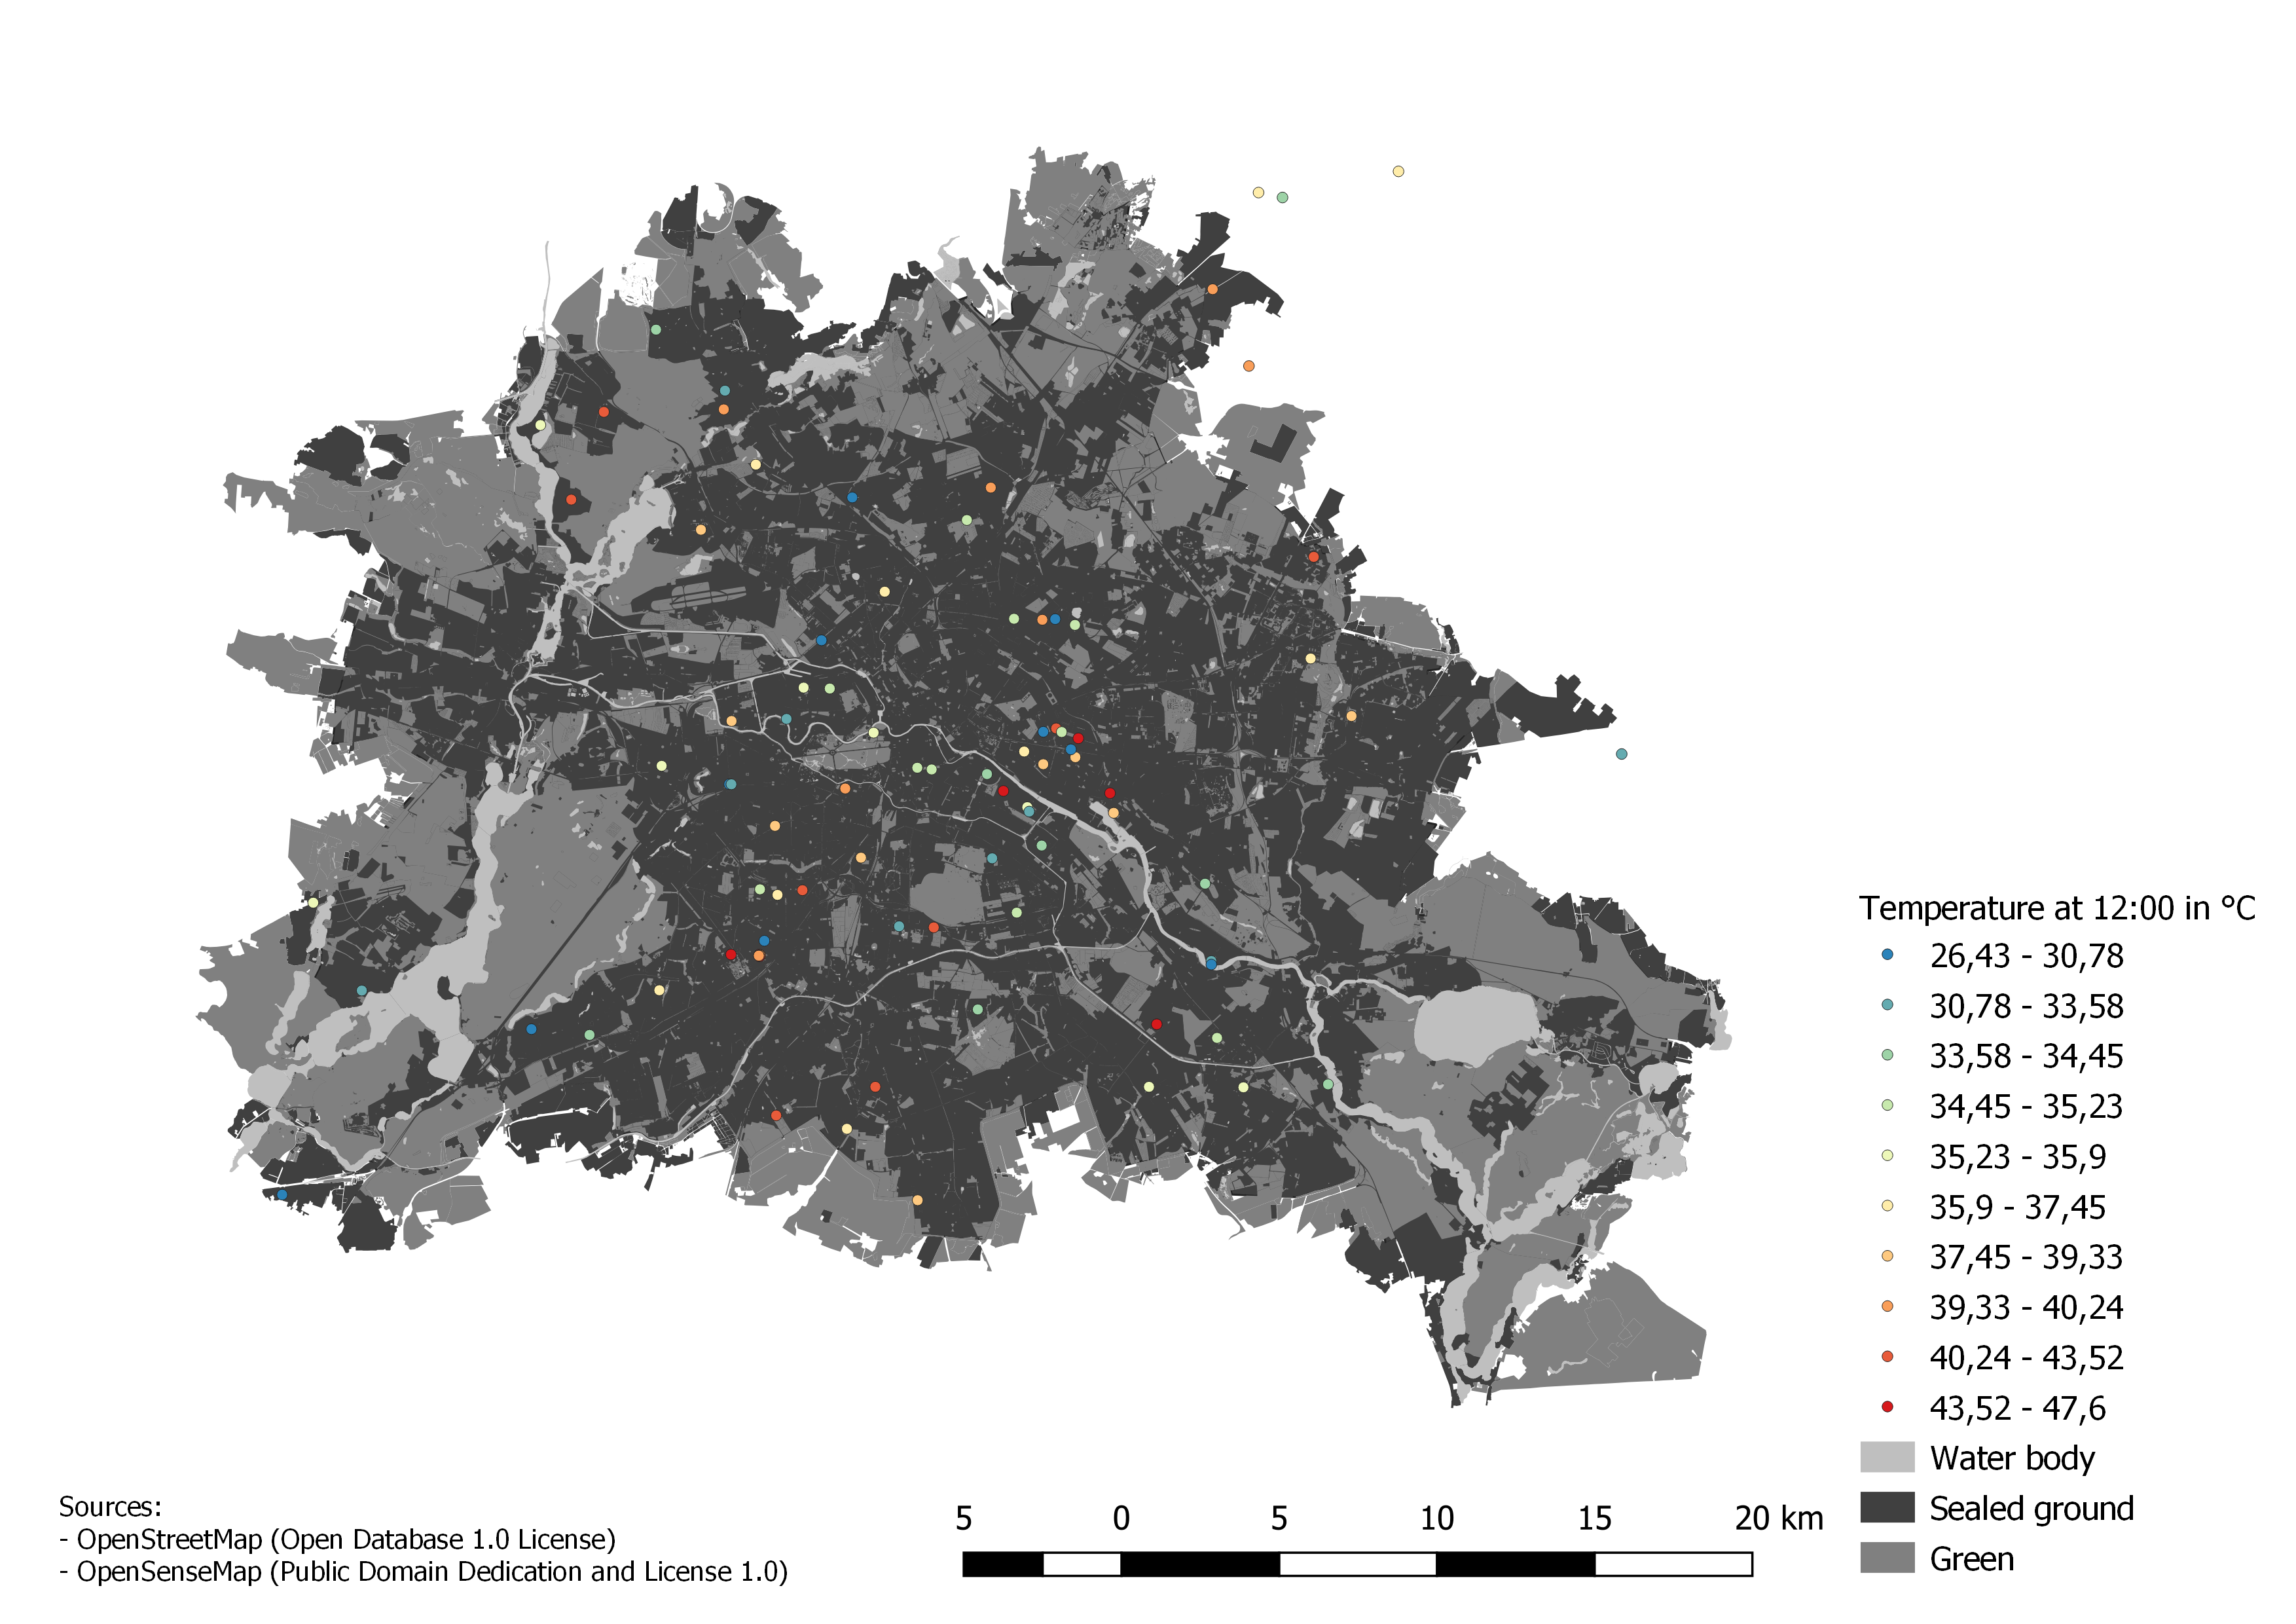
\includegraphics[width=\linewidth]{comparison/berlin.png}
	\caption{Surface types and sensor locations in research area}
	\label{fig:result_berlin}
\end{figure}

\subsection{Nearest neighbor}

The method \ldq{}Nearest neighbor\rdq{} is displayed by smaller regions (cells) with sharp edges  (see figure \ref{fig:result_nearest}). Its distinctive visual characteristics do not give sophisticated information about the temperature distribution within the city of Berlin. The geometric shapes of the regions only give a general idea of where the heat islands are, but it does not allow a detailed analysis of the effect nor does provide a precise location/center of the occurring heat.

\begin{figure}
	\centering
	\subfloat[\centering Nearest neighbor interpolation using GDAL\label{fig:result_nearest}]{{\includegraphics[width=.48\linewidth]{images/interpolation_nearest.png} }}
	\hfill
	\subfloat[\centering TIN interpolation using GDAL\label{fig:result_linear}]{{\includegraphics[width=.48\linewidth]{images/interpolation_tin.png} }}
	\caption{Nearest neighbor and TIN interpolation using GDAL in comparison}
	\label{fig:result_nearest_linear}
\end{figure}


\subsection{TIN interpolation}

Figure \ref{fig:result_linear} shows the results of the TIN interpolation. Hereby visible is the characteristic surface made of triangles and the sharp edges. The fact that TIN interpolation was used to create the image can easily be seen due to the visible convex hull. Due to visual examination the underlying calculation based on the relationship with the nodes of the triangles are apparent. The IUHI is not sufficiently depicted and is not very detailed and, therefore, does not provide enough information.


\subsection{IDW interpolation}

For the IDW interpolation, GDAL and GRASS GIS were used in order to be able to compare the results. Visually, IDW is recognizable by the \ldq{}Bull Eyes\rdq{}-effect. These are concentric areas of equal values, which can be seen around the known points or stations. Compared to the Nearest neighbor and TIN interpolation methods, IDW gives a much more detailed output and allows for distinctive analysis of the temperature distribution. Both, the calculation with GDAL and GRASS, give similar results as shown in figure \ref{fig:result_idw_gdal_grass}. Although the prominent points are fairly similar, differences can be seen in more sparsely covered areas.

\begin{figure}
	\centering
	\subfloat[\centering IDW interpolation using GDAL\label{fig:result_idw_gdal}]{{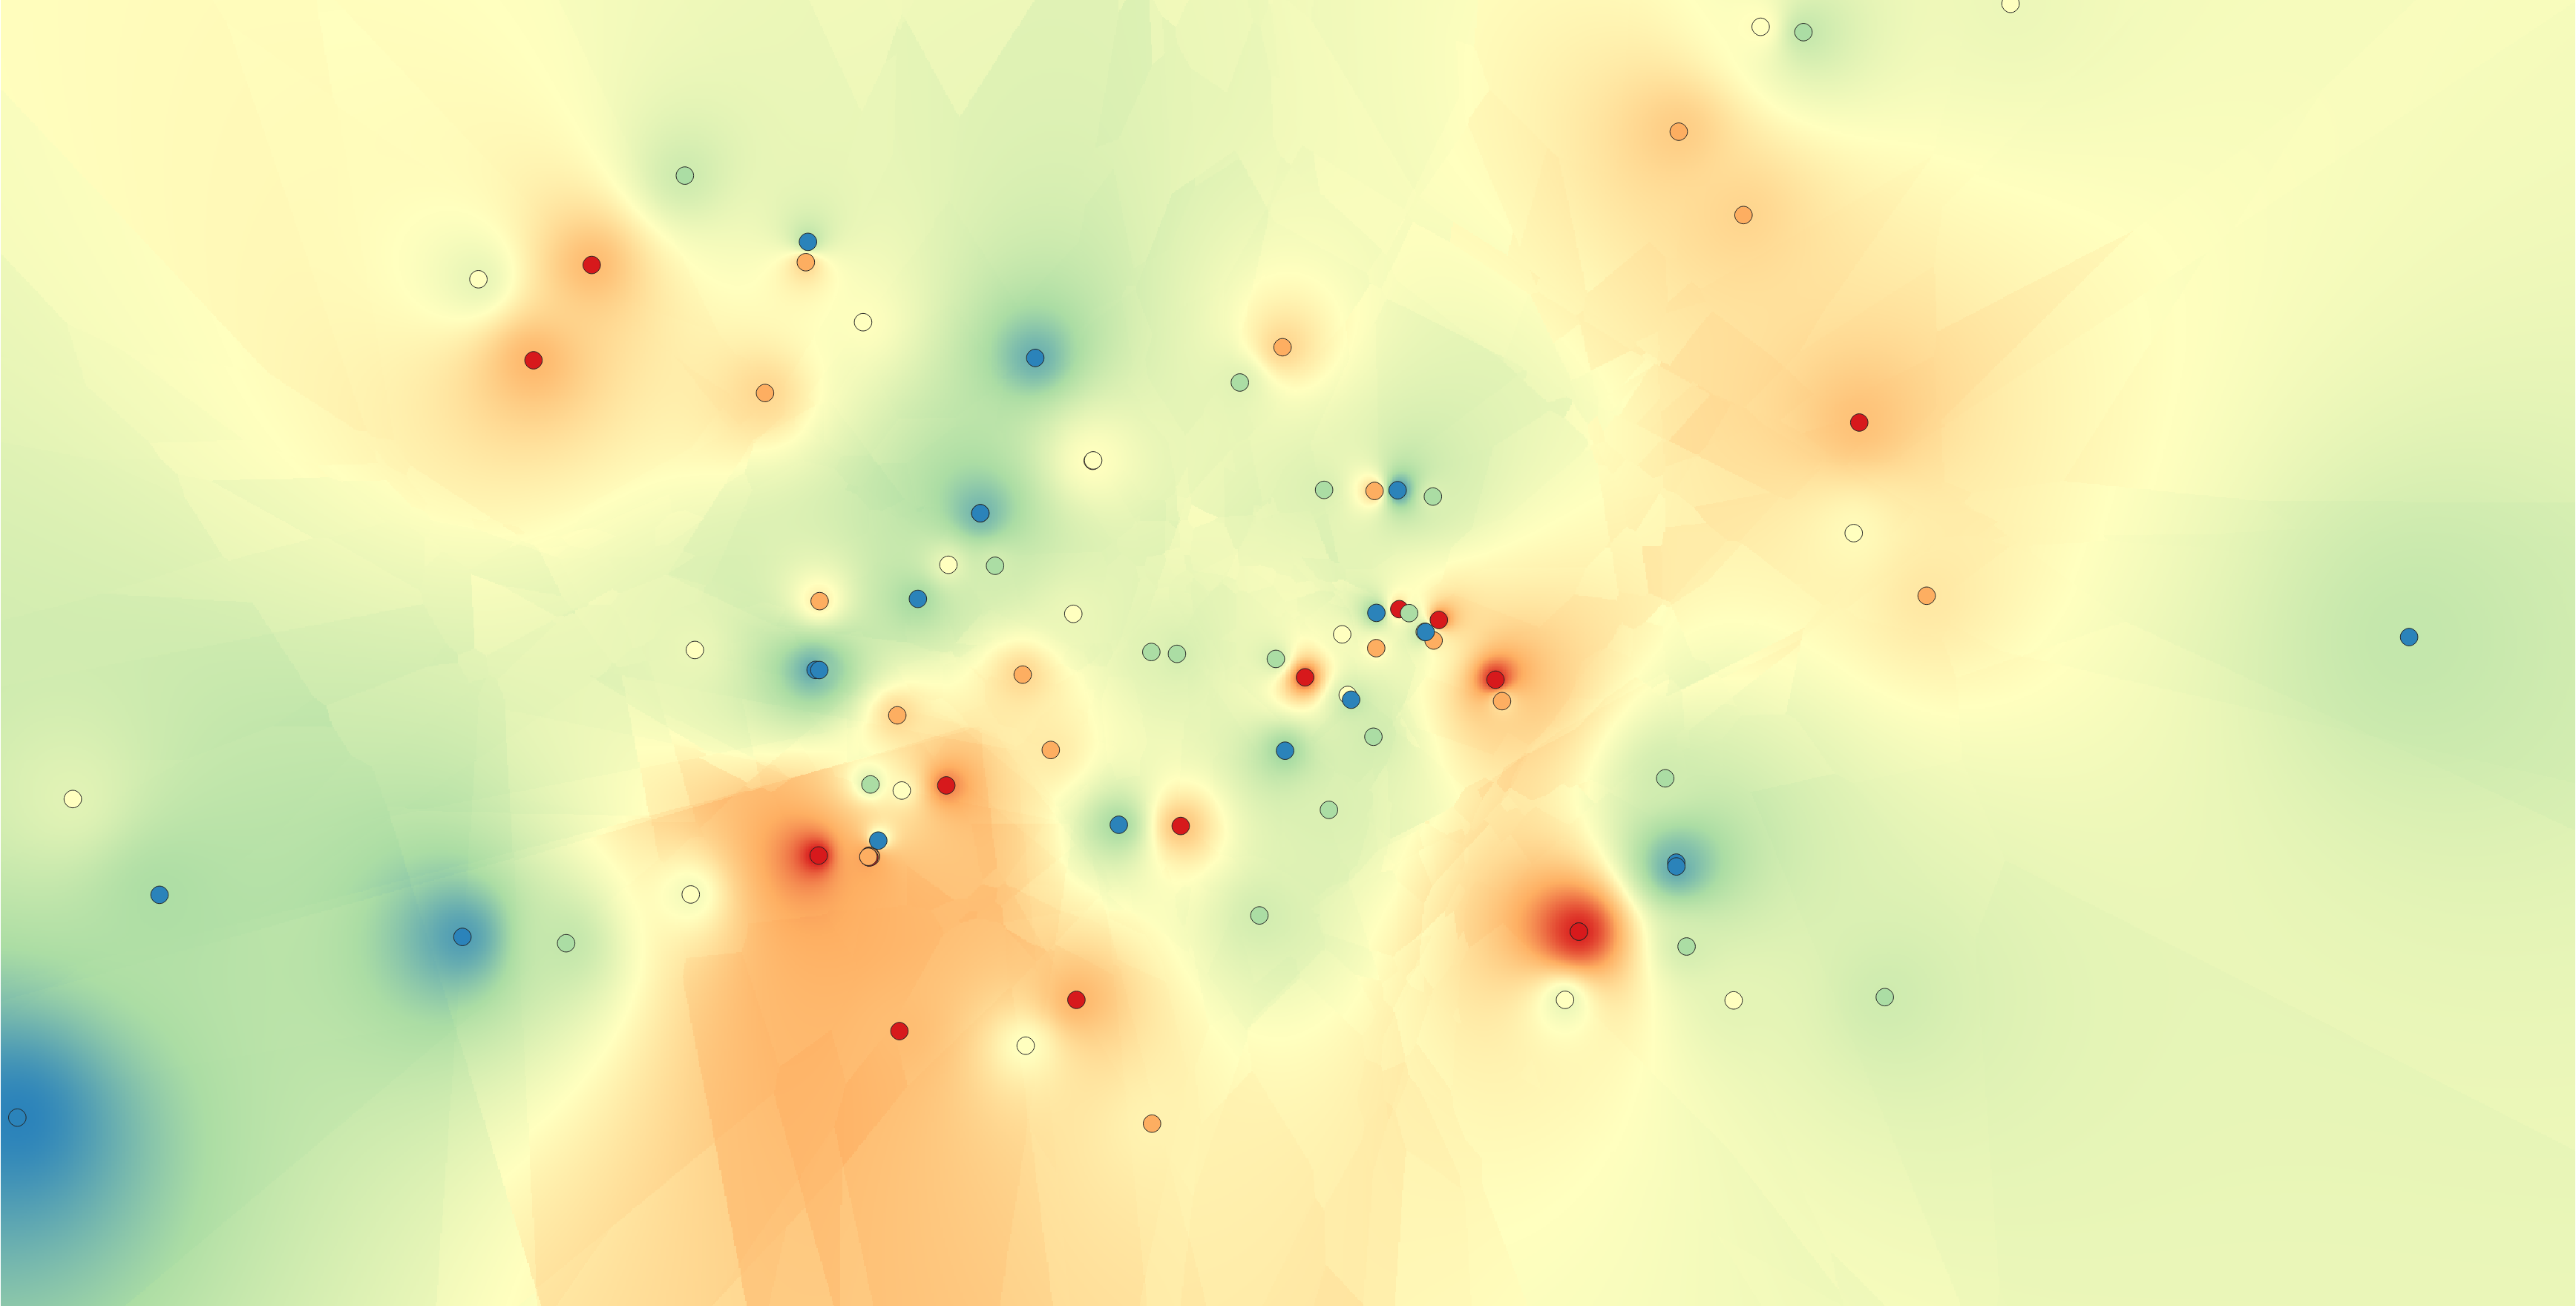
\includegraphics[width=.48\linewidth]{comparison/compare_idw_gdal.png} }}
	\hfill
	\subfloat[\centering IDW interpolation using GRASS GIS\label{fig:result_idw_grass}]{{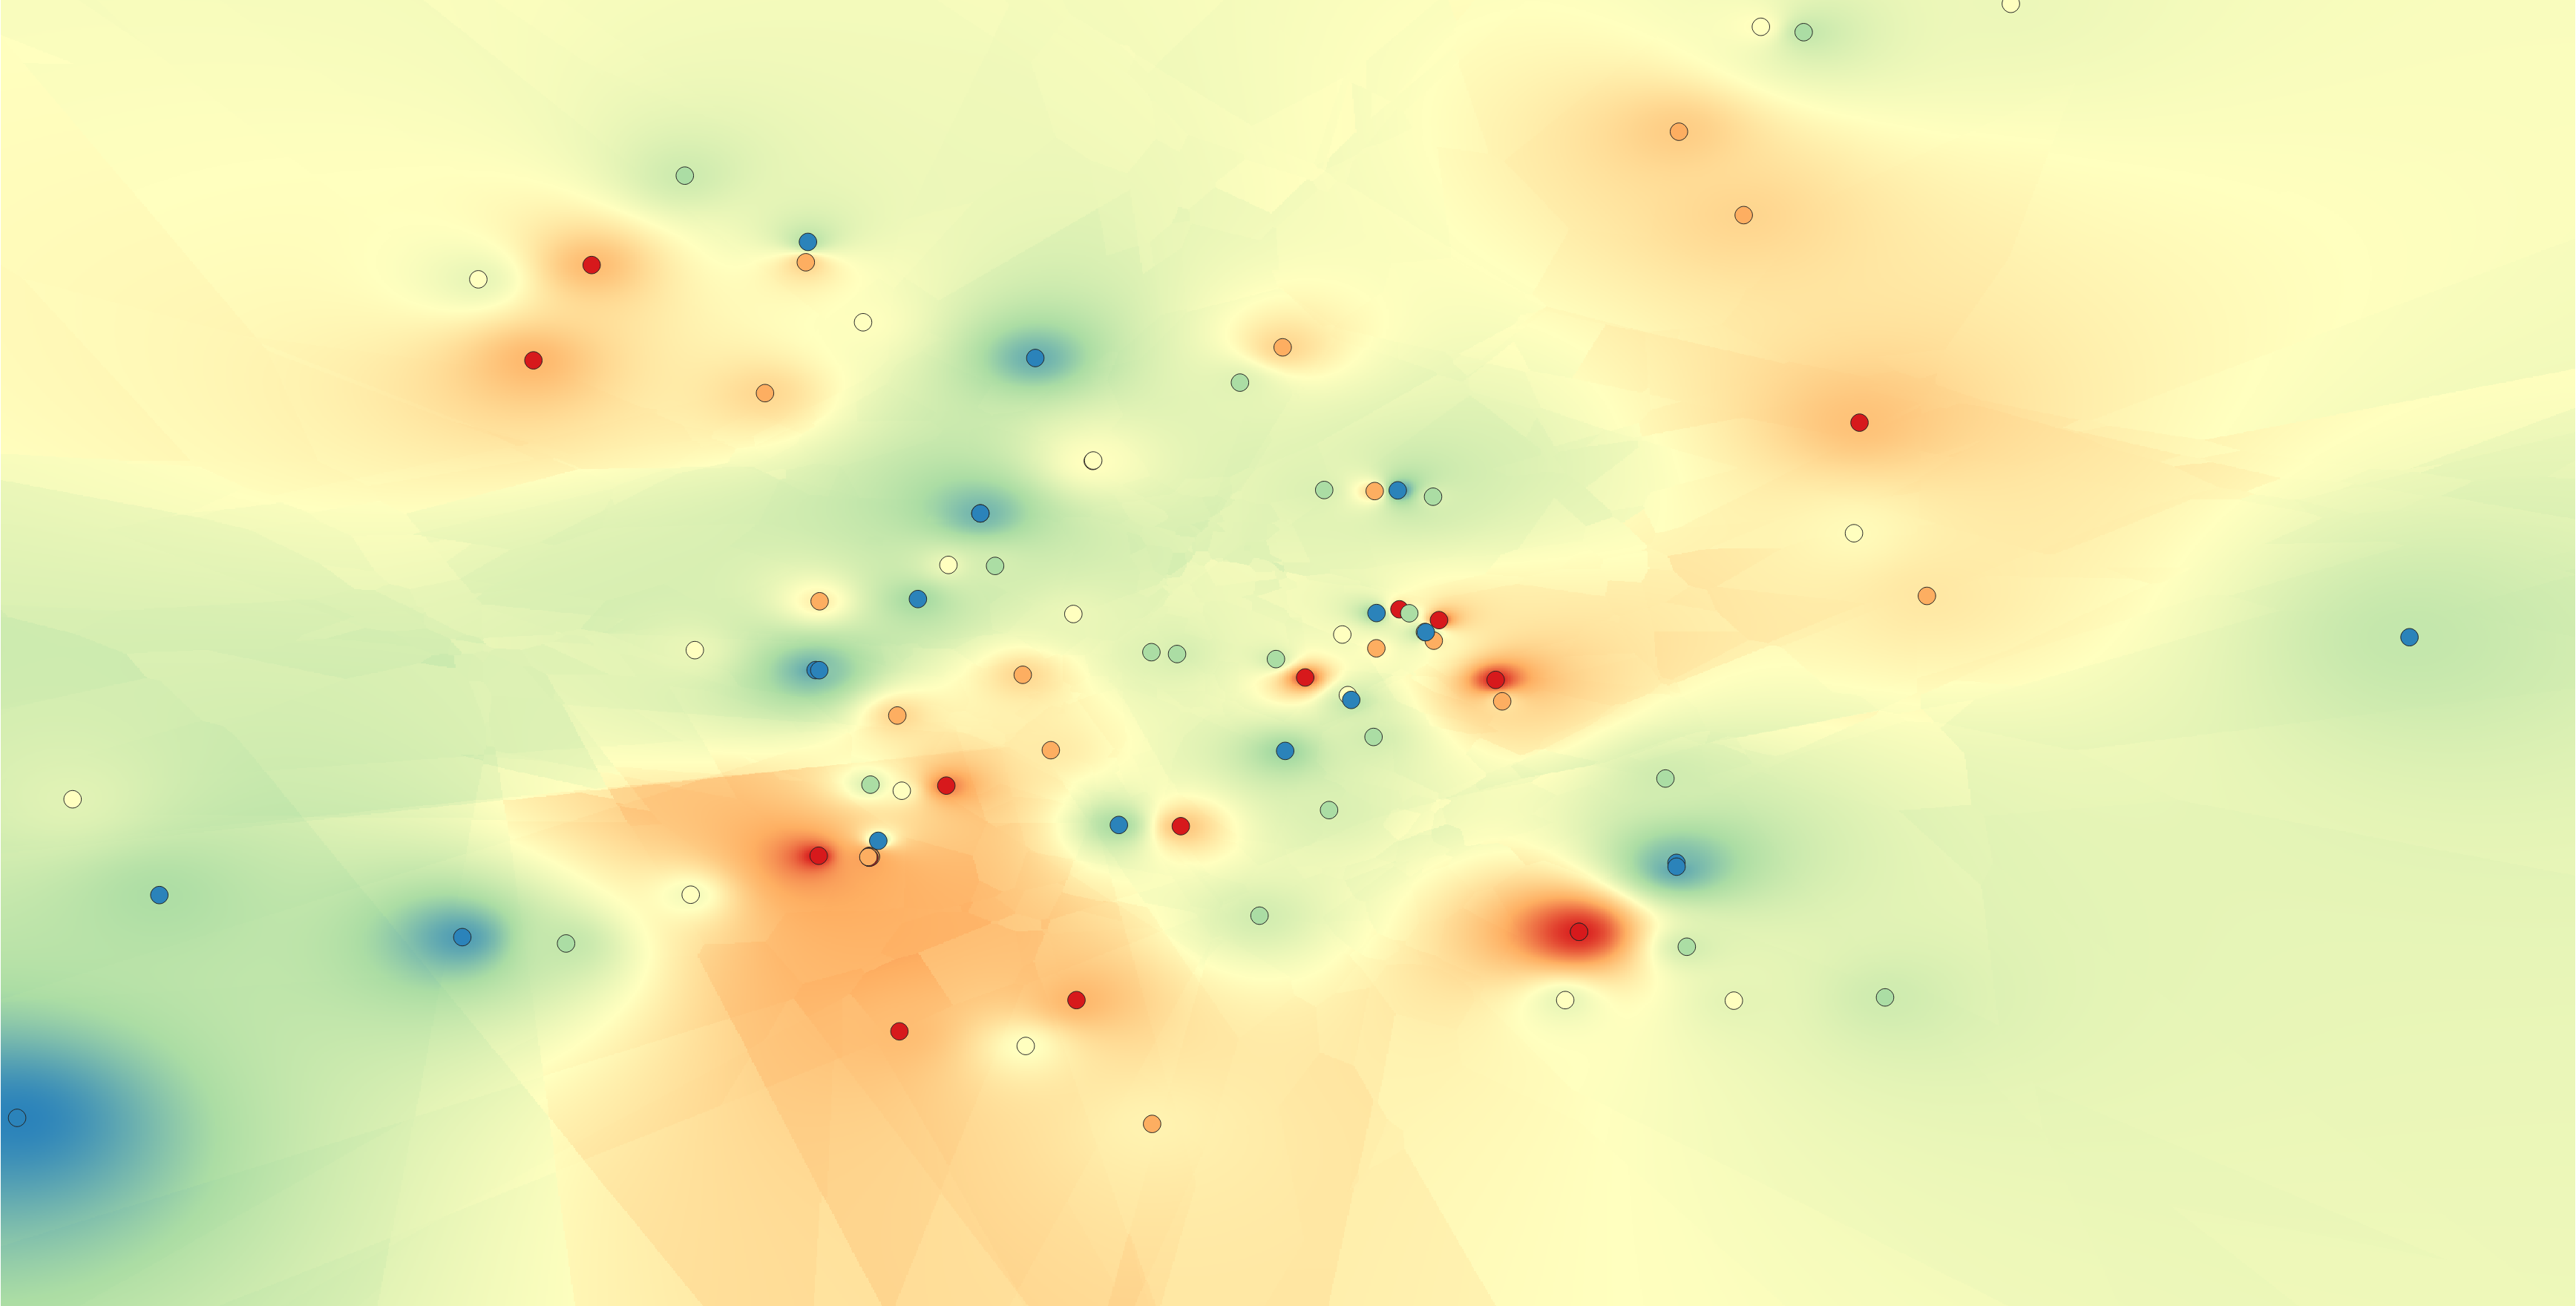
\includegraphics[width=.48\linewidth]{comparison/compare_idw_grass.png} }}
	\caption[Comparison of IDW interpolation between GDAL and GRASS GIS]{Comparison of IDW interpolation between GDAL and GRASS GIS, both using 12 max neighbors and a power factor of 2}
	\label{fig:result_idw_gdal_grass}
\end{figure}

\subsection{B-Spline interpolation}

As SAGA GIS also offers the possibility to interpolate point data, we conducted a B-Spline approximation. SAGA was identified as being one of the least accurate methods as illustrated by \citeauthor{wenjing_cao_study_2009}. As argued before, data points, which are not evenly distributed and have large value differences could pose a problem for Spline interpolation. The result seems to have been \ldq{}smoothed\rdq{} out heavily and thus display a very homogeneous data surface. Figure \ref{fig:result_bspline} shows that temperature distributions have a farther reaching impact (compare lower left corner as well as the rightmost station with IDW). The smoothness can be seen on multiple clusters where, in contrast, the IDW interpolation creates islands that aren't interconnected and the IDW results show more fringed edges.

\begin{figure}[H]
	\centering
	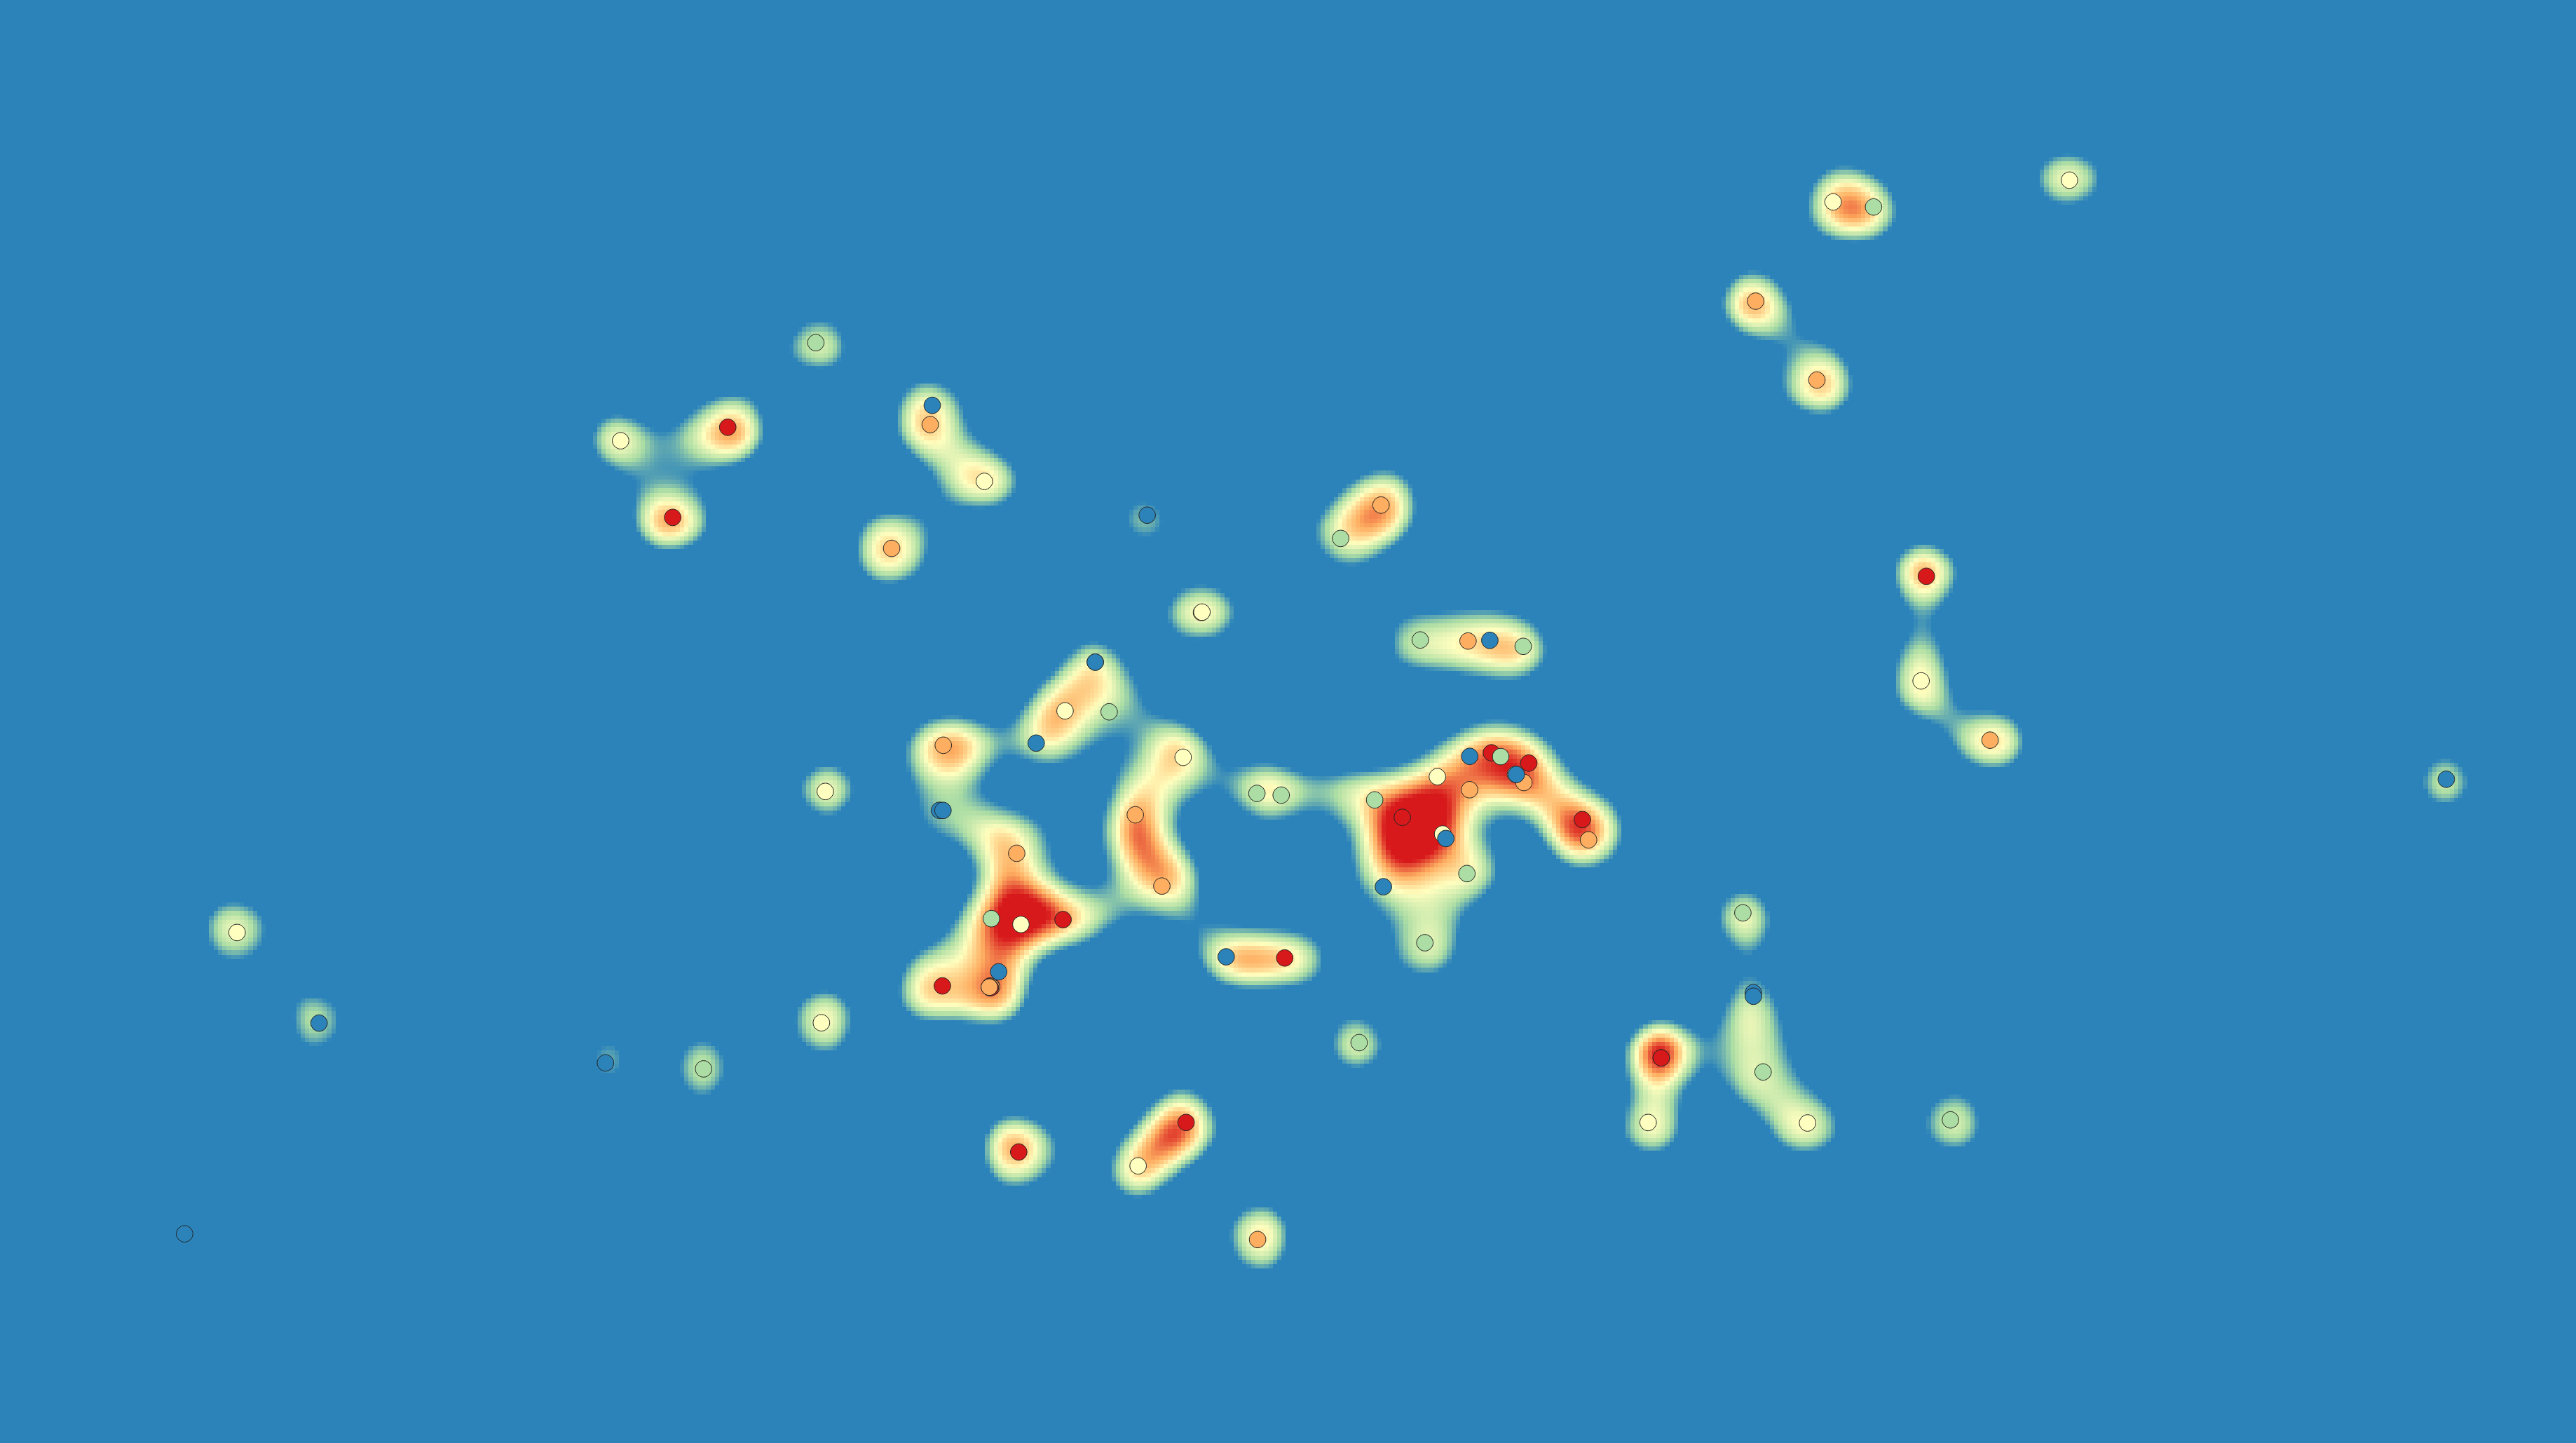
\includegraphics[width=.7\linewidth]{comparison/compare_bspline_saga.png}
	\caption{B-Spline interpolation using SAGA GIS}
	\label{fig:result_bspline}
\end{figure}
